\documentclass{standalone}
\usepackage{tikz}
\usetikzlibrary{patterns, positioning}


\begin{document}
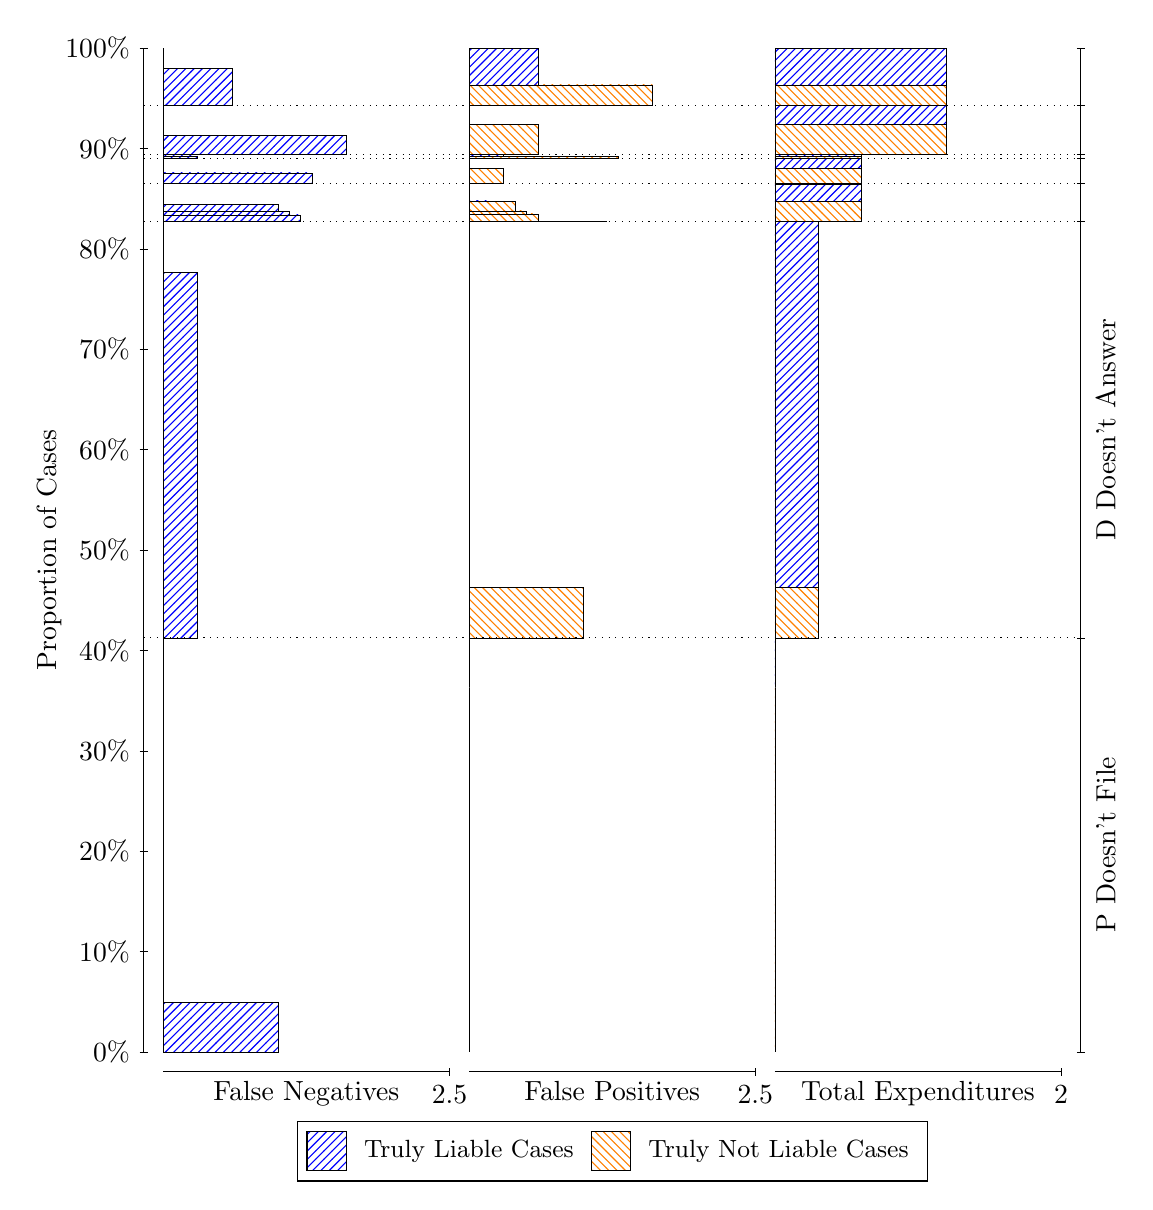
\begin{tikzpicture}
\draw[black, very thin] (1.5,1.75) -- (1.5,14.5);
\node[rotate=90, text=black, anchor=center] at (0.3, 8.125) {Proportion of Cases};
\draw[black, very thin] (1.45,1.75) -- (1.55,1.75);
\node[text=black, anchor=east] at (1.45, 1.75) {0\%};
\draw[black, very thin] (1.45,3.025) -- (1.55,3.025);
\node[text=black, anchor=east] at (1.45, 3.025) {10\%};
\draw[black, very thin] (1.45,4.3) -- (1.55,4.3);
\node[text=black, anchor=east] at (1.45, 4.3) {20\%};
\draw[black, very thin] (1.45,5.575) -- (1.55,5.575);
\node[text=black, anchor=east] at (1.45, 5.575) {30\%};
\draw[black, very thin] (1.45,6.85) -- (1.55,6.85);
\node[text=black, anchor=east] at (1.45, 6.85) {40\%};
\draw[black, very thin] (1.45,8.125) -- (1.55,8.125);
\node[text=black, anchor=east] at (1.45, 8.125) {50\%};
\draw[black, very thin] (1.45,9.4) -- (1.55,9.4);
\node[text=black, anchor=east] at (1.45, 9.4) {60\%};
\draw[black, very thin] (1.45,10.675) -- (1.55,10.675);
\node[text=black, anchor=east] at (1.45, 10.675) {70\%};
\draw[black, very thin] (1.45,11.95) -- (1.55,11.95);
\node[text=black, anchor=east] at (1.45, 11.95) {80\%};
\draw[black, very thin] (1.45,13.225) -- (1.55,13.225);
\node[text=black, anchor=east] at (1.45, 13.225) {90\%};
\draw[black, very thin] (1.45,14.5) -- (1.55,14.5);
\node[text=black, anchor=east] at (1.45, 14.5) {100\%};

\draw[black, very thin] (13.4,1.75) -- (13.4,14.5);
\draw[black, very thin] (13.35,1.75) -- (13.45,1.75);
\node[anchor=west] at (13.35, 1.75) {};
\draw[black, very thin] (13.35,7.01) -- (13.45,7.01);
\node[anchor=west] at (13.35, 7.01) {};
\draw[black, very thin] (13.35,12.295) -- (13.45,12.295);
\node[anchor=west] at (13.35, 12.295) {};
\draw[black, very thin] (13.35,12.78) -- (13.45,12.78);
\node[anchor=west] at (13.35, 12.78) {};
\draw[black, very thin] (13.35,13.102) -- (13.45,13.102);
\node[anchor=west] at (13.35, 13.102) {};
\draw[black, very thin] (13.35,13.146) -- (13.45,13.146);
\node[anchor=west] at (13.35, 13.146) {};
\draw[black, very thin] (13.35,13.771) -- (13.45,13.771);
\node[anchor=west] at (13.35, 13.771) {};
\draw[black, very thin] (13.35,14.5) -- (13.45,14.5);
\node[anchor=west] at (13.35, 14.5) {};

\draw[black, very thin, pattern color=blue, pattern=north east lines] (1.75,1.75) rectangle (3.2033,2.3828);
\draw[black, very thin, pattern color=orange, pattern=north west lines] (1.75,2.3828) rectangle (1.75,7.01);
\draw[black, very thin, pattern color=blue, pattern=north east lines] (1.75,7.01) rectangle (2.186,11.655);
\draw[black, very thin, pattern color=orange, pattern=north west lines] (1.75,11.655) rectangle (1.75,12.295);
\draw[black, very thin, pattern color=blue, pattern=north east lines] (1.75,12.295) rectangle (3.494,12.38);
\draw[black, very thin, pattern color=blue, pattern=north east lines] (1.75,12.38) rectangle (3.3487,12.421);
\draw[black, very thin, pattern color=blue, pattern=north east lines] (1.75,12.421) rectangle (3.2033,12.512);
\draw[black, very thin, pattern color=blue, pattern=north east lines] (1.75,12.512) rectangle (3.058,12.512);
\draw[black, very thin, pattern color=blue, pattern=north east lines] (1.75,12.512) rectangle (3.058,12.513);
\draw[black, very thin, pattern color=blue, pattern=north east lines] (1.75,12.513) rectangle (2.9127,12.514);
\draw[black, very thin, pattern color=blue, pattern=north east lines] (1.75,12.514) rectangle (2.7673,12.515);
\draw[black, very thin, pattern color=blue, pattern=north east lines] (1.75,12.515) rectangle (2.622,12.516);
\draw[black, very thin, pattern color=blue, pattern=north east lines] (1.75,12.516) rectangle (2.4767,12.517);
\draw[black, very thin, pattern color=blue, pattern=north east lines] (1.75,12.517) rectangle (2.3313,12.519);
\draw[black, very thin, pattern color=orange, pattern=north west lines] (1.75,12.519) rectangle (1.75,12.78);
\draw[black, very thin, pattern color=blue, pattern=north east lines] (1.75,12.78) rectangle (3.6393,12.914);
\draw[black, very thin, pattern color=orange, pattern=north west lines] (1.75,12.914) rectangle (1.75,13.102);
\draw[black, very thin, pattern color=blue, pattern=north east lines] (1.75,13.102) rectangle (2.186,13.129);
\draw[black, very thin, pattern color=orange, pattern=north west lines] (1.75,13.129) rectangle (1.75,13.146);
\draw[black, very thin, pattern color=blue, pattern=north east lines] (1.75,13.146) rectangle (4.0753,13.391);
\draw[black, very thin, pattern color=orange, pattern=north west lines] (1.75,13.391) rectangle (1.75,13.771);
\draw[black, very thin, pattern color=blue, pattern=north east lines] (1.75,13.771) rectangle (2.622,14.239);
\draw[black, very thin, pattern color=orange, pattern=north west lines] (1.75,14.239) rectangle (1.75,14.5);
\draw[black, very thin, pattern color=orange, pattern=north west lines] (5.6333,1.75) rectangle (5.6333,6.3773);
\draw[black, very thin, pattern color=blue, pattern=north east lines] (5.6333,6.3773) rectangle (5.6333,7.01);
\draw[black, very thin, pattern color=orange, pattern=north west lines] (5.6333,7.01) rectangle (7.0867,7.6499);
\draw[black, very thin, pattern color=blue, pattern=north east lines] (5.6333,7.6499) rectangle (5.6333,12.295);
\draw[black, very thin, pattern color=orange, pattern=north west lines] (5.6333,12.295) rectangle (7.3773,12.297);
\draw[black, very thin, pattern color=orange, pattern=north west lines] (5.6333,12.297) rectangle (7.232,12.297);
\draw[black, very thin, pattern color=orange, pattern=north west lines] (5.6333,12.297) rectangle (7.0867,12.298);
\draw[black, very thin, pattern color=orange, pattern=north west lines] (5.6333,12.298) rectangle (6.9413,12.299);
\draw[black, very thin, pattern color=orange, pattern=north west lines] (5.6333,12.299) rectangle (6.796,12.3);
\draw[black, very thin, pattern color=orange, pattern=north west lines] (5.6333,12.3) rectangle (6.6507,12.301);
\draw[black, very thin, pattern color=orange, pattern=north west lines] (5.6333,12.301) rectangle (6.5053,12.393);
\draw[black, very thin, pattern color=orange, pattern=north west lines] (5.6333,12.393) rectangle (6.36,12.433);
\draw[black, very thin, pattern color=orange, pattern=north west lines] (5.6333,12.433) rectangle (6.2147,12.557);
\draw[black, very thin, pattern color=blue, pattern=north east lines] (5.6333,12.557) rectangle (5.924,12.559);
\draw[black, very thin, pattern color=blue, pattern=north east lines] (5.6333,12.559) rectangle (5.7787,12.56);
\draw[black, very thin, pattern color=blue, pattern=north east lines] (5.6333,12.56) rectangle (5.6333,12.78);
\draw[black, very thin, pattern color=orange, pattern=north west lines] (5.6333,12.78) rectangle (6.0693,12.968);
\draw[black, very thin, pattern color=blue, pattern=north east lines] (5.6333,12.968) rectangle (5.6333,13.102);
\draw[black, very thin, pattern color=orange, pattern=north west lines] (5.6333,13.102) rectangle (7.5227,13.119);
\draw[black, very thin, pattern color=blue, pattern=north east lines] (5.6333,13.119) rectangle (6.0693,13.146);
\draw[black, very thin, pattern color=orange, pattern=north west lines] (5.6333,13.146) rectangle (6.5053,13.526);
\draw[black, very thin, pattern color=blue, pattern=north east lines] (5.6333,13.526) rectangle (5.6333,13.771);
\draw[black, very thin, pattern color=orange, pattern=north west lines] (5.6333,13.771) rectangle (7.9587,14.032);
\draw[black, very thin, pattern color=blue, pattern=north east lines] (5.6333,14.032) rectangle (6.5053,14.5);
\draw[black, very thin, pattern color=orange, pattern=north west lines] (9.5167,1.75) rectangle (9.5167,6.3773);
\draw[black, very thin, pattern color=blue, pattern=north east lines] (9.5167,6.3773) rectangle (9.5167,7.01);
\draw[black, very thin, pattern color=orange, pattern=north west lines] (9.5167,7.01) rectangle (10.062,7.6499);
\draw[black, very thin, pattern color=blue, pattern=north east lines] (9.5167,7.6499) rectangle (10.062,12.295);
\draw[black, very thin, pattern color=orange, pattern=north west lines] (9.5167,12.295) rectangle (10.607,12.298);
\draw[black, very thin, pattern color=blue, pattern=north east lines] (9.5167,12.298) rectangle (10.607,12.3);
\draw[black, very thin, pattern color=orange, pattern=north west lines] (9.5167,12.3) rectangle (10.607,12.556);
\draw[black, very thin, pattern color=blue, pattern=north east lines] (9.5167,12.556) rectangle (10.607,12.773);
\draw[black, very thin, pattern color=orange, pattern=north west lines] (9.5167,12.773) rectangle (10.607,12.776);
\draw[black, very thin, pattern color=blue, pattern=north east lines] (9.5167,12.776) rectangle (10.607,12.78);
\draw[black, very thin, pattern color=orange, pattern=north west lines] (9.5167,12.78) rectangle (10.607,12.968);
\draw[black, very thin, pattern color=blue, pattern=north east lines] (9.5167,12.968) rectangle (10.607,13.102);
\draw[black, very thin, pattern color=orange, pattern=north west lines] (9.5167,13.102) rectangle (10.607,13.119);
\draw[black, very thin, pattern color=blue, pattern=north east lines] (9.5167,13.119) rectangle (10.607,13.146);
\draw[black, very thin, pattern color=orange, pattern=north west lines] (9.5167,13.146) rectangle (11.697,13.526);
\draw[black, very thin, pattern color=blue, pattern=north east lines] (9.5167,13.526) rectangle (11.697,13.771);
\draw[black, very thin, pattern color=orange, pattern=north west lines] (9.5167,13.771) rectangle (11.697,14.032);
\draw[black, very thin, pattern color=blue, pattern=north east lines] (9.5167,14.032) rectangle (11.697,14.5);
\draw[black, dotted] (1.5,7.01) -- (13.4,7.01);
\draw[black, dotted] (1.5,12.295) -- (13.4,12.295);
\draw[black, dotted] (1.5,12.78) -- (13.4,12.78);
\draw[black, dotted] (1.5,13.102) -- (13.4,13.102);
\draw[black, dotted] (1.5,13.146) -- (13.4,13.146);
\draw[black, dotted] (1.5,13.771) -- (13.4,13.771);
\draw[black, very thin] (1.75,1.5) -- (5.3833,1.5);
\node[text=black, anchor=north] at (3.5667, 1.5) {False Negatives};
\draw[black, very thin] (5.3833,1.45) -- (5.3833,1.55);
\node[text=black, anchor=north] at (5.3833, 1.45) {2.5};

\draw[black, very thin] (5.6333,1.5) -- (9.2667,1.5);
\node[text=black, anchor=north] at (7.45, 1.5) {False Positives};
\draw[black, very thin] (9.2667,1.45) -- (9.2667,1.55);
\node[text=black, anchor=north] at (9.2667, 1.45) {2.5};

\draw[black, very thin] (9.5167,1.5) -- (13.15,1.5);
\node[text=black, anchor=north] at (11.333, 1.5) {Total Expenditures};
\draw[black, very thin] (13.15,1.45) -- (13.15,1.55);
\node[text=black, anchor=north] at (13.15, 1.45) {2};

\node[text=black, centered, rotate=90] at (13.72, 4.38) {P Doesn't File};
\node[text=black, centered, rotate=90] at (13.72, 9.6526) {D Doesn't Answer};






\draw (7.449999999999999,1.5) node[draw=none] (baseCoordinate) {};
\begin{scope}[align=center]
        \matrix[scale=0.5, draw=black, below=0.5cm of baseCoordinate, nodes={draw}, column sep=0.1cm]{
            \node[rectangle, draw, minimum width=0.5cm, minimum height=0.5cm, pattern color=blue, pattern=north east lines] {}; &
            \node[draw=none, font=\small, text=black] (B) {Truly Liable Cases}; &
            \node[rectangle, draw, minimum width=0.5cm, minimum height=0.5cm, pattern color=orange, pattern=north west lines] {}; &
            \node[draw=none, font=\small, text=black] (B) {Truly Not Liable Cases}; \\
            };
\end{scope}

\end{tikzpicture}
\end{document}